\clearpage
\section{New Frontend for SAFE Server} 
\hspace{0.5cm} 

\subsection{Problem Statement}
	Create a new frontend for the SAFE server, which is intuitive and easy to use

\subsection{Why do we need this?}
	The current UI/UX of the SAFE server was difficult to understand and use. Also the Industrial Design Centre (IDC) in IIT reviewed SAFE and gave a low Usability score. It was necessary to create a new Frontend which adhered to the common UX patterns and make it easy even for a new user to use the system. 

\subsection{Design}
	Multiple brainstorming sessions were done to identify the pain points in the current Server and how these can be fixed. We have also gone through the UI/UX guidelines of Google and Facebook and made sure the new frontend adhered to these guidelines and best practices. Care was taken to reduce the number of clicks the user has to do to execute some action. Color schemes was also fixed so that there is a uniform look and feel throughout the site.

\subsection{Implementation}
	After much dicussion the following Pages were finalized

    \begin{itemize}
        \item Dashboard - Shows list of currently running quizzes, recent quiz instances and quizzes and courses
	    \item Course page with following subpages
	    \begin{itemize}
	        \item Quizzes page - Shows all the quizzes in the given quiz along with quiz access buttons for frequent actions like running a quiz, editing a quiz etc.
		    \item Settings page - View / Edit Course Settings
	    \end{itemize}
		
	    \item Quiz Page
	    \begin{itemize}
	        \item Questions page - View all the questions in the quiz along with quiz settings
		    \item Quiz edit page - Create / Edit questions in a quiz in a Google forms like interface using drag and drop
		    \item Settings page - View / Edit quiz settings
		    \item Instances - Run new instances of quiz
		    \item Quiz live Dashboard - See live statistics about a running quiz and alerts
		    \item Submissions - Unified page to see both partial submissions and final submissions of different instances. 
		    \item Statistics - Statistics for the quiz
	    \end{itemize}
	\end{itemize}

	A fully working prototype (not linked with the actual server, runs on dummy data, but fully fuctional) was created using a bootstrap based opensource Admin template - AdminLTE along with custom CSS. AngularJS v1.6 was used as the javascript library since it allows quick prototyping for the complex interaction which were required for the new design. After creating the initial prototype we did 4 iterations of usability testing and refinements to ensure that any issues found are fixed.
 
\subsection{Screenshots}

\begin{figure}[h!]
\begin{center}
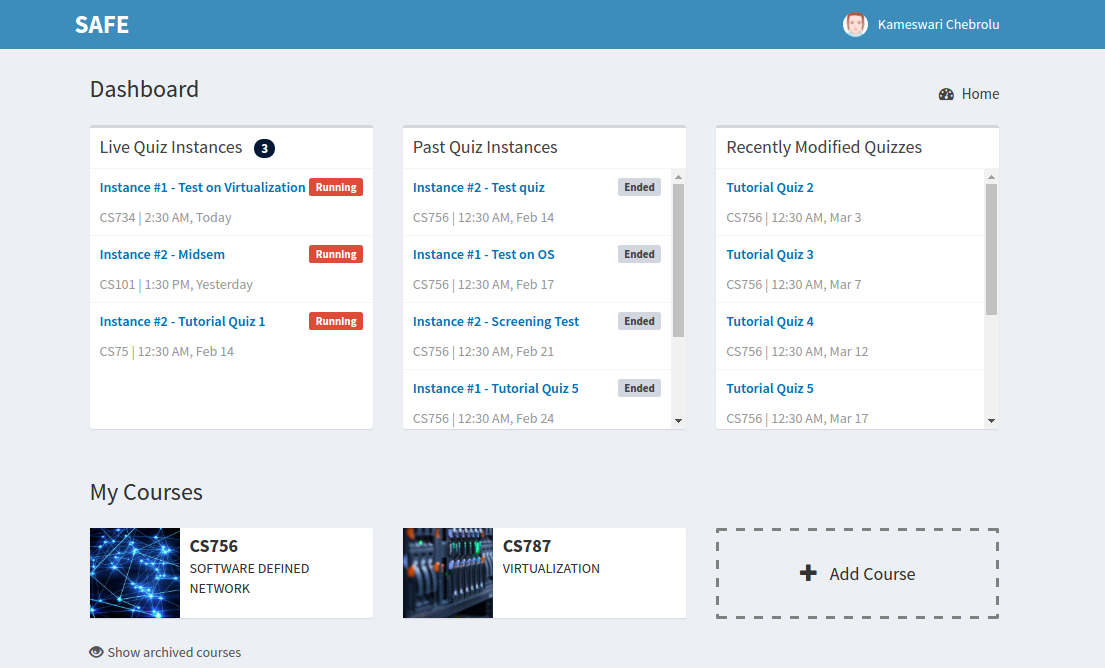
\includegraphics[scale=.4]{diagrams/new-ui-1} 
\vspace{1cm}
\caption{Dashboard Page}
\end{center}
\end{figure}


\begin{figure}[h!]
\begin{center}
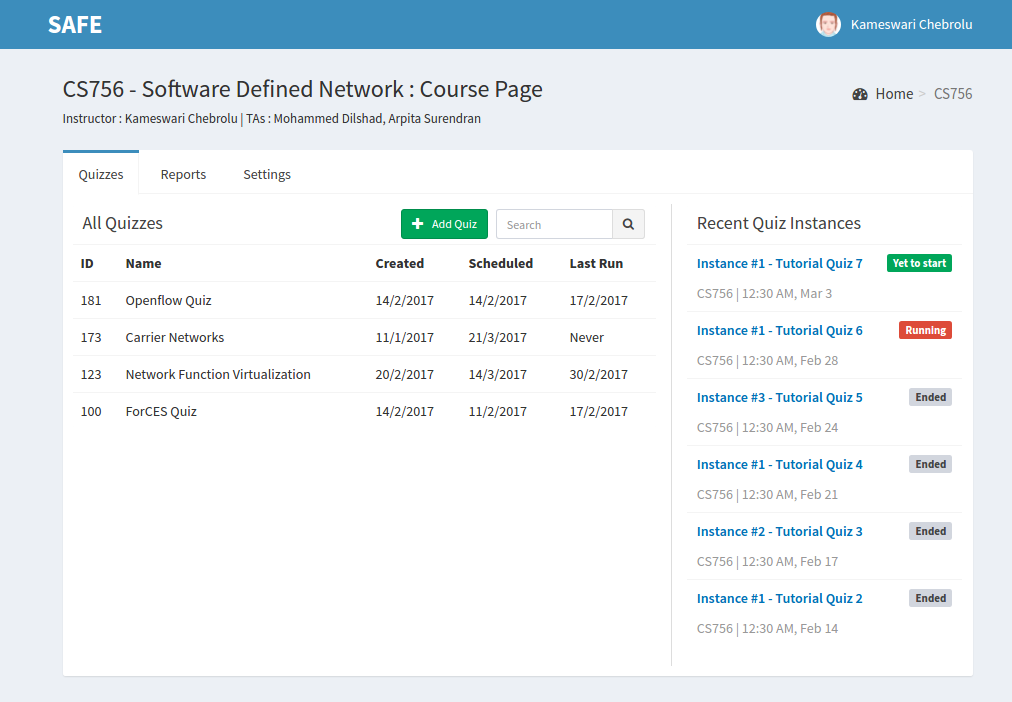
\includegraphics[scale=.35]{diagrams/new-ui-2} 
\caption{Course Page}
\end{center}
\end{figure}

\begin{figure}[h!]
\begin{center}
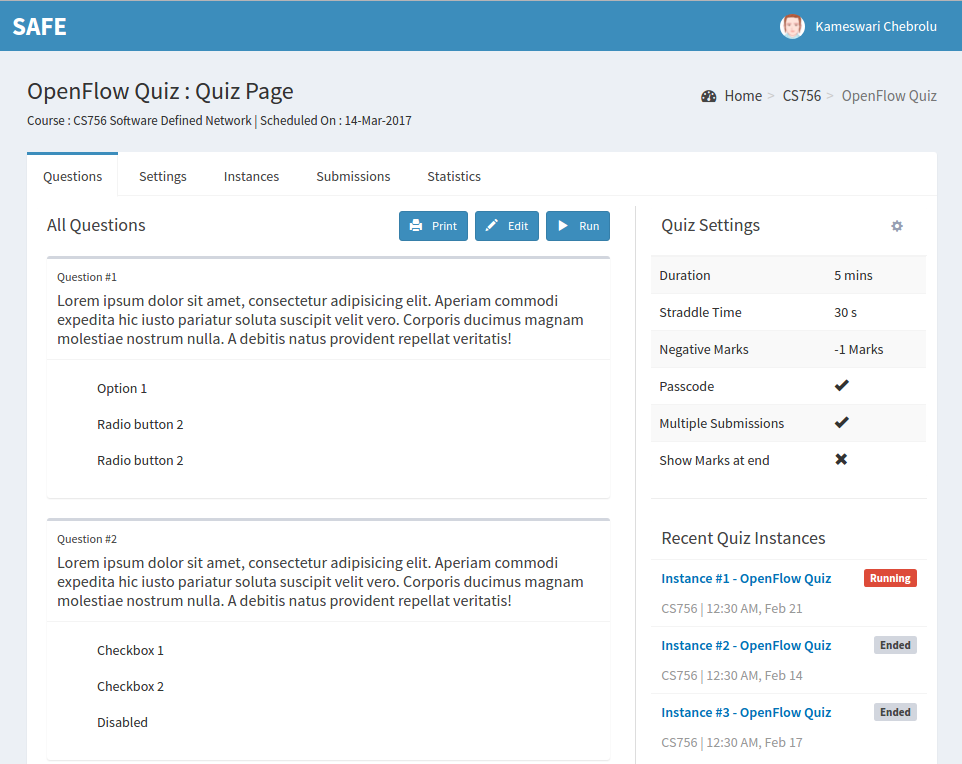
\includegraphics[scale=.35]{diagrams/new-ui-3} 
\caption{Quiz Questions Page}
\end{center}
\end{figure}

\begin{figure}[h!]
\begin{center}
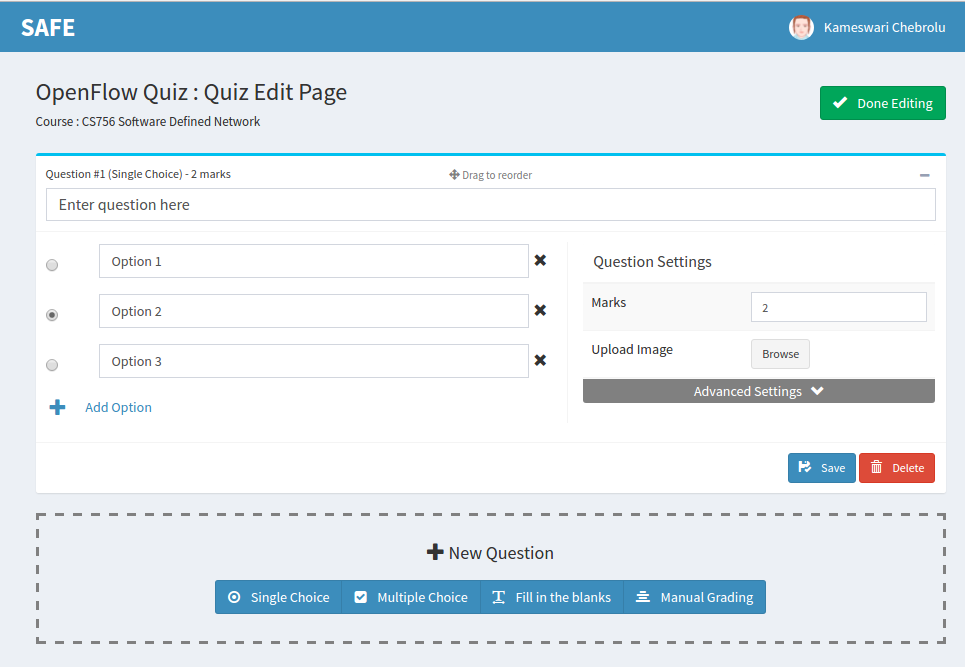
\includegraphics[scale=.4]{diagrams/new-ui-4} 
\caption{Quiz Edit Page}
\end{center}
\end{figure}

\begin{figure}[h!]
\begin{center}
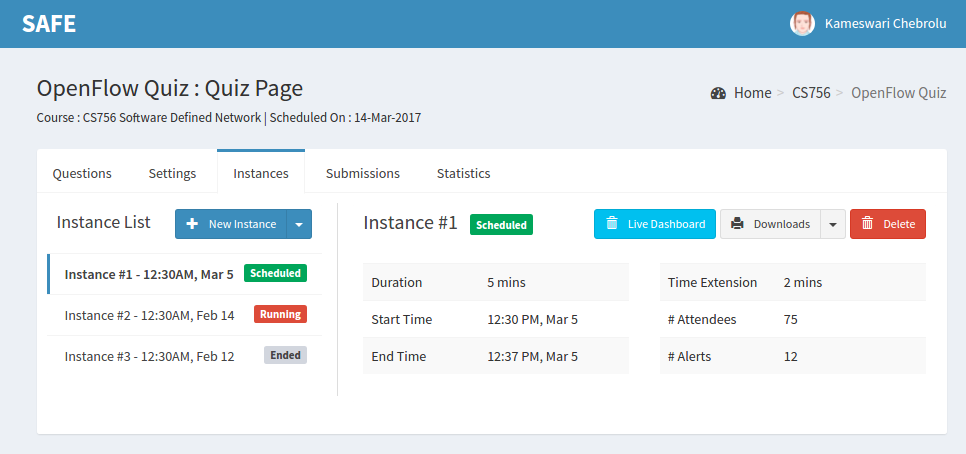
\includegraphics[scale=.4]{diagrams/new-ui-5} 
\caption{Quiz Instances Page}
\end{center}
\end{figure}

